%\documentclass{article}
%\usepackage[utf8]{inputenc}
%\usepackage{tikz}
%\usepackage{amsmath}
\usetikzlibrary{positioning}

%\begin{document}

%------------------------------------------------------------------------------
% QSPK

%\begin{figure}
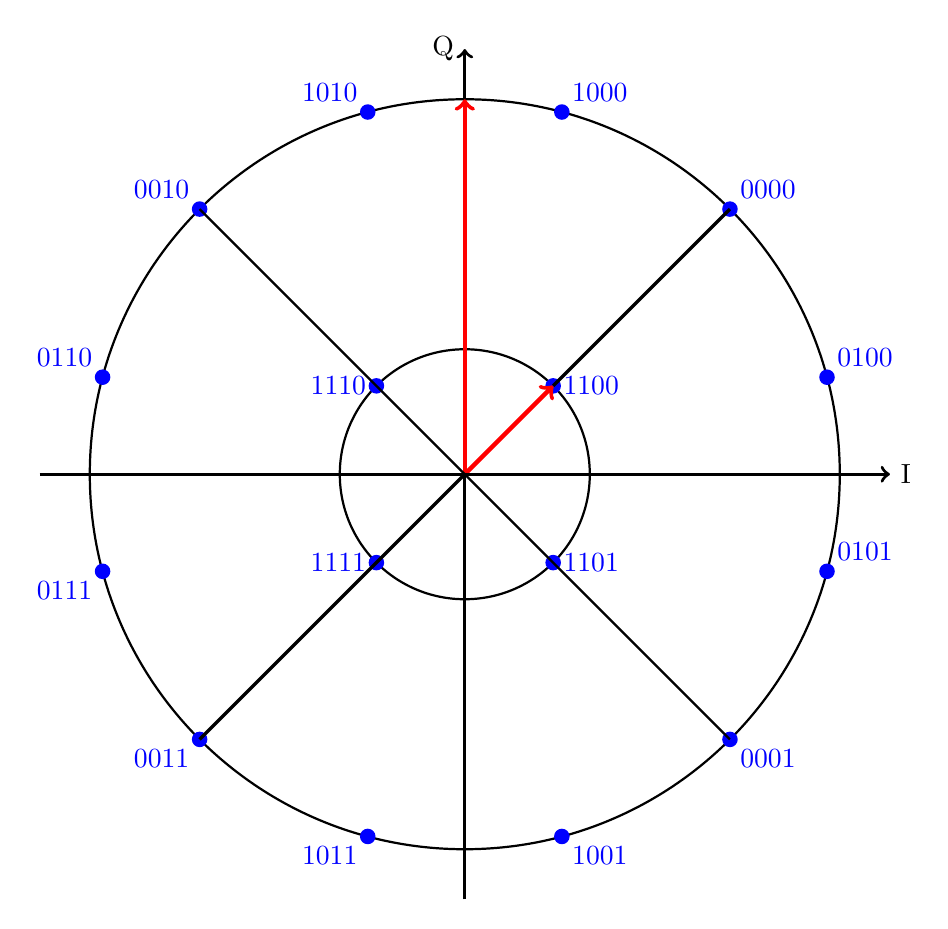
\begin{tikzpicture}[thick,scale=0.6]


%-------------------Inner Circle--------------------%
\draw[thick](0,0) circle (2.64575131);

\filldraw [blue] (2.64575131*0.707106781,2.64575131*0.707106781) circle (4pt) node[anchor=west] {1100};
\filldraw [blue] (2.64575131*-0.707106781,2.64575131*0.707106781) circle (4pt) node[anchor=east] {1110};
\filldraw [blue] (2.64575131*-0.707106781,2.64575131*-0.707106781) circle (4pt) node[anchor=east] {1111};
\filldraw [blue] (2.64575131*0.707106781,2.64575131*-0.707106781) circle (4pt) node[anchor=west] {1101};
\draw[red,ultra thick,->] (0,0) -- (2.64575131*0.707106781,2.64575131*0.707106781);
%----------------------------------------------------%


%-------------------External Circle-----------------%
\draw[thick](0,0) circle (3*2.64575131);
%----------------------Q1-----------------%
\filldraw [blue] (3*2.64575131*0.965925826,3*2.64575131*0.258819045) circle (4pt) node[anchor=south west] {0100};
\filldraw [blue] (3*2.64575131*0.707106781,3*2.64575131*0.707106781) circle (4pt) node[anchor=south west] {0000};
\filldraw [blue] (3*2.64575131*0.258819045,3*2.64575131*0.965925826) circle (4pt) node[anchor=south west] {1000};
%----------------------Q2-----------------%
\filldraw [blue] (3*2.64575131*-0.258819045,3*2.64575131*0.965925826) circle (4pt) node[anchor=south east] {1010};
\filldraw [blue] (3*2.64575131*-0.707106781,3*2.64575131*0.707106781) circle (4pt) node[anchor=south east] {0010};
\filldraw [blue] (3*2.64575131*-0.965925826,3*2.64575131*0.258819045) circle (4pt) node[anchor=south east] {0110};
%----------------------Q3-----------------%
\filldraw [blue] (3*2.64575131*-0.965925826,3*2.64575131*-0.258819045) circle (4pt) node[anchor=north east] {0111};
\filldraw [blue] (3*2.64575131*-0.707106781,3*2.64575131*-0.707106781) circle (4pt) node[anchor=north east] {0011};
\filldraw [blue] (3*2.64575131*-0.258819045,3*2.64575131*-0.965925826) circle (4pt) node[anchor=north east] {1011};
%----------------------Q4-----------------%
\filldraw [blue] (3*2.64575131*0.258819045,3*2.64575131*-0.965925826) circle (4pt) node[anchor=north west] {1001};
\filldraw [blue] (3*2.64575131*0.707106781,3*2.64575131*-0.707106781) circle (4pt) node[anchor=north west] {0001};
\filldraw [blue] (3*2.64575131*0.965925826,3*2.64575131*-0.258819045) circle (4pt) node[anchor=south west] {0101};
%----------------------------------------------------%

\draw[red,ultra thick,->] (0,0) -- (0,3*2.64575131);
\draw[black,very thick,->] (-9,0) -- (9,0) node[anchor=west] {I};
\draw[black,very thick] (0,-9) -- (0,0) ;
\draw[black,very thick] (2.64575131*0.707106781,2.64575131*0.707106781) -- (3*2.64575131*0.707106781,3*2.64575131*0.707106781) ;
\draw[black,very thick] (0,0) -- (3*2.64575131*-0.707106781,3*2.64575131*-0.707106781) ;
\draw[black,thick] (3*2.64575131*-0.707106781,3*2.64575131*0.707106781) -- (3*2.64575131*0.707106781,3*2.64575131*-0.707106781) ;
\draw[black,very thick,->] (0,3*2.64575131) -- (0,9) node[anchor=east] {Q};
\end{tikzpicture}
%\end{figure}

%\begin{equation*}
%$X_k \in \cbrak{X}$=
%\begin{cases}
%$r_1 e^{j\brak{\phi_1+\frac{2\pi}{4}n}}& n=0,\dots,3$\\
%$r_2 e^{j\brak{\phi_2+\frac{2\pi}{12}n}}& n=0,1,\dots,11$
%\end{cases}
%\end{equation*}
%------------------------------------------------------------------------------

%\end{document}
